%
% teil2.tex -- perfekt geradlinige Bewegung
%
% (c) 2020 Prof Dr Andreas Müller, Hochschule Rapperswil
%
% !TEX root = ../../buch.tex
% !TEX encoding = UTF-8
%
\section{Perfekte geradlinige Bewegung
\label{geradlinig:section:perfekte_geradlinige}}
\kopfrechts{Perfekte geradlinige Bewegung}
Im 19.\,Jahrhundert wurde mathematisch gezeigt, 
dass ein Viergelenkmechanismus keine perfekte geradlinige 
Bewegung erzeugen kann.
Davor entwickelte Pierre Frédéric Sarrus einen Mechanismus, 
\index{Sarrus, Pierre Frederic@Sarrus, Pierre Frédéric}%
der das Problem mit sechs Gelenken löste.
Dieser Mechanismus ist in Abbildung~\ref{fig:sarrus_link} dargestellt.
Seine Erfindung erhielt jedoch nur wenig Aufmerksamkeit.
Ein möglicher Grund dafür war, dass es sich nicht um einen planaren, 
sondern um einen räumlichen Mechanismus handelte.
Dadurch war die Konstruktion für praktische Anwendungen weniger geeignet.
\begin{figure}
    \centering
    \begin{minipage}{0.32\textwidth}
        \centering
        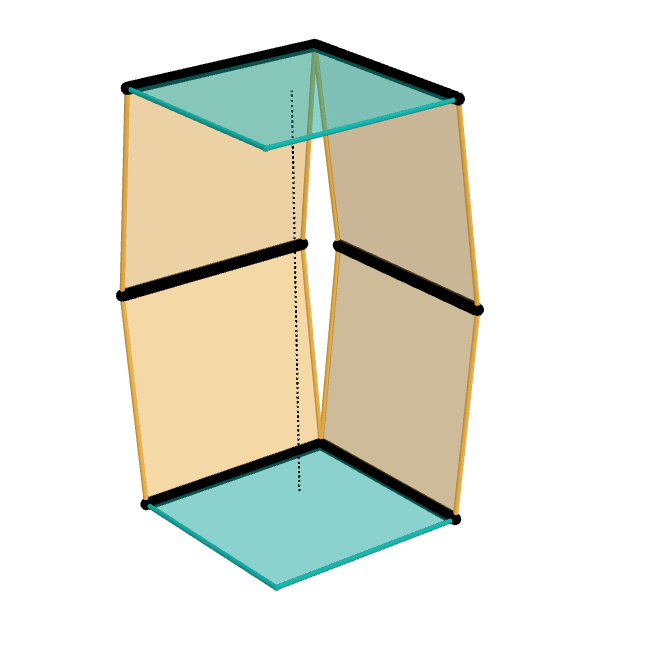
\includegraphics[width=\textwidth]{papers/geradlinig/figures/sarrus_linkage1.png}
    \end{minipage}
    \hfill
    \begin{minipage}{0.32\textwidth}
        \centering
        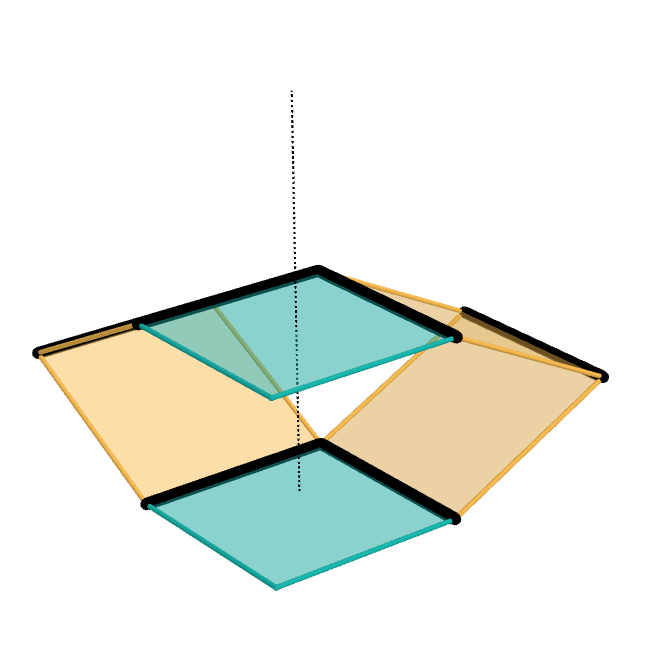
\includegraphics[width=\textwidth]{papers/geradlinig/figures/sarrus_linkage2.png}
    \end{minipage}
    \hfill
    \begin{minipage}{0.32\textwidth}
        \centering
        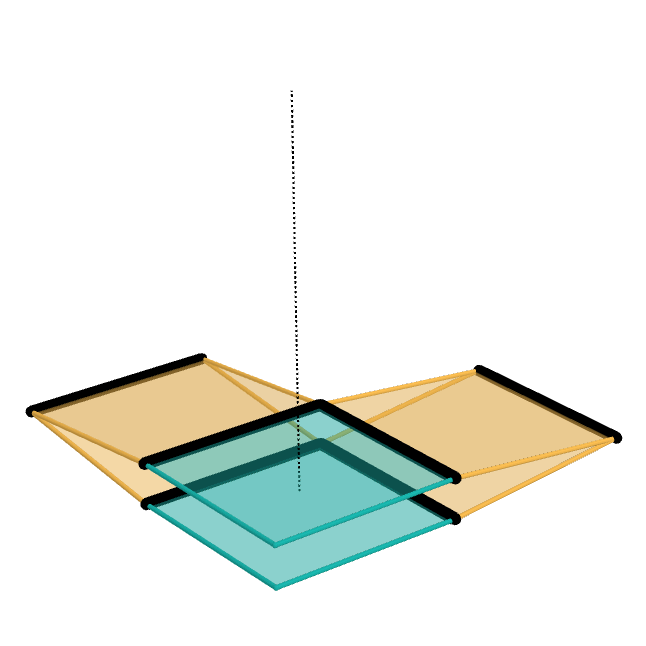
\includegraphics[width=\textwidth]{papers/geradlinig/figures/sarrus_linkage3.png}
    \end{minipage}
    \caption{Der Mechanismus von Sarrus~\cite{sarrus_linkage}.}
    \label{fig:sarrus_link}
\end{figure}


Im Jahr 1864 entwickelte Charles-Nicolas Peaucellier den ersten 
\index{Peaucellier, Charles-Nicolas}%
planaren Mechanismus, welcher eine Rotationsbewegung in 
eine perfekte geradlinige Bewegung umwandeln konnte.
Der Mechanismus ist in Abbildung~\ref{fig:peaucellier_link} dargestellt.
Einige Jahre später entwickelte Yom Tov Lipman Lipkin 
\index{Lipkin, Yom Tov Lipman}%
unabhängig denselben Mechanismus.
Zu Ehren beider Erfinder wird dieser als 
Peaucellier-Lipkin-Mechanismus bezeichnet.
\index{Peaucellier-Lipkin-Mechanismus}%
Um dieses geometrische Phänomen besser zu verstehen,
müssen wir zuerst die Theorie der Kreisspiegelung entwickeln.
\index{Kreisspiegelung}%
Diese wird im kommenden Abschnitt genauer behandelt
sowie auch der Zusammenhang mit der komplexen Ebene.
\begin{figure}
    \centering
    \begin{minipage}{0.32\textwidth}
        \centering
        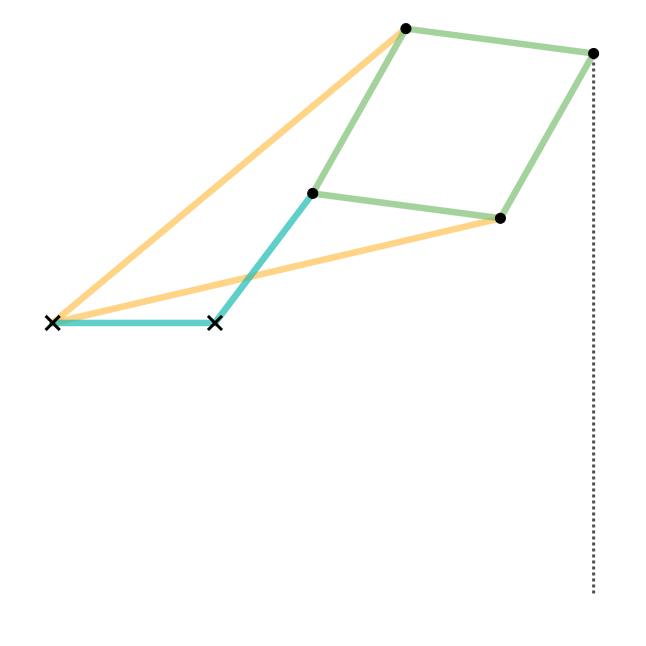
\includegraphics[width=\textwidth]{papers/geradlinig/figures/peaucellier_linkage1.png}
    \end{minipage}
    \hfill
    \begin{minipage}{0.32\textwidth}
        \centering
        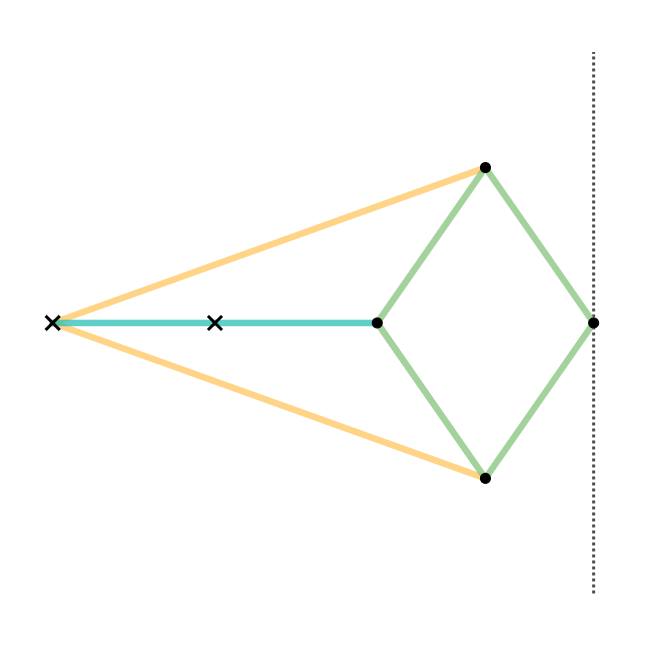
\includegraphics[width=\textwidth]{papers/geradlinig/figures/peaucellier_linkage2.png}
    \end{minipage}
    \hfill
    \begin{minipage}{0.32\textwidth}
        \centering
        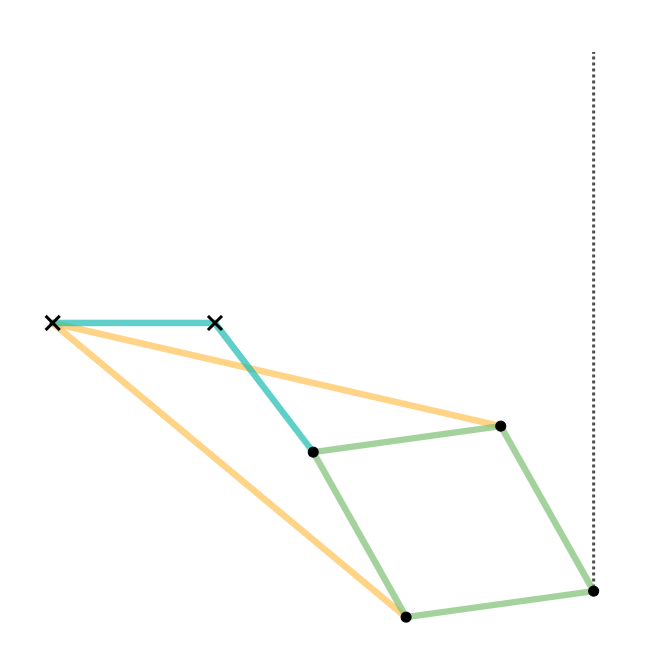
\includegraphics[width=\textwidth]{papers/geradlinig/figures/paucellier_linkage3.png}
    \end{minipage}
    \caption{Der Mechanismus von Peaucellier und Lipkin~\cite{peauc_lip_linkage}.}
    \label{fig:peaucellier_link}
\end{figure}

